\documentclass{article}
\usepackage{tikz}
\usepackage{geometry}
\usepackage{fancyhdr}
\usepackage{enumitem}
\usepackage{amsmath}
\usepackage{hyperref}

\geometry{letterpaper, left=1cm, right=1cm, top=2cm, bottom=2cm}

\pagestyle{fancy}
\fancyhf{}
\renewcommand{\headrulewidth}{0pt}
\fancyfoot[LE,RO]{\thepage}
\fancyfoot[RE,LO]{\copyright\hspace{0.25em}codeabode 2025. \href{https://codeabode.co}{\underline{codeabode.co}}}

\title{\vspace{-3em}Coordinate Plane Worksheet\vspace{-2em}}
\date{}

\begin{document}

\maketitle

\section*{Instructions:}
For each problem below, plot the given points or movements on the coordinate plane. Then write the final coordinate(s) in the answer box. Each grid line represents 0.5 units.

\begin{enumerate}
    \item Plot the point (3, -3) on the coordinate plane below.
    
    \begin{center}
    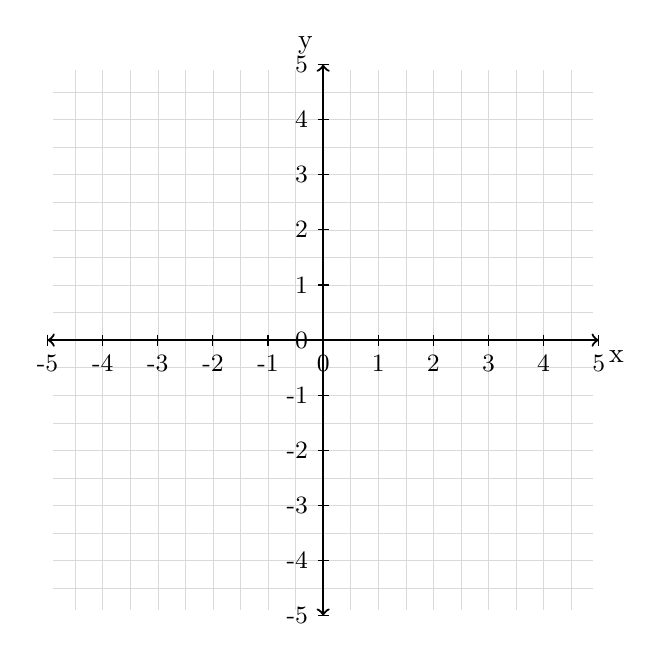
\begin{tikzpicture}[scale=0.7]
        \draw[gray!30, very thin, step=0.5] (-4.9,-4.9) grid (4.9,4.9);
        \draw[thick, <->] (-5,0) -- (5,0) node[below right] {x};
        \draw[thick, <->] (0,-5) -- (0,5) node[above left] {y};
        \foreach \x in {-5,-4,...,5} {
            \draw (\x,0.1) -- (\x,-0.1) node[below] {\small\x};
        }
        \foreach \y in {-5,-4,...,5} {
            \draw (0.1,\y) -- (-0.1,\y) node[left] {\small\y};
        }
    \end{tikzpicture}
    \end{center}
    
    Final coordinate: \rule{3cm}{0.4pt}
    
    \item Plot the points (2.5, 0.5) and (-1, -2.5) on the coordinate plane below.
    
    \begin{center}
    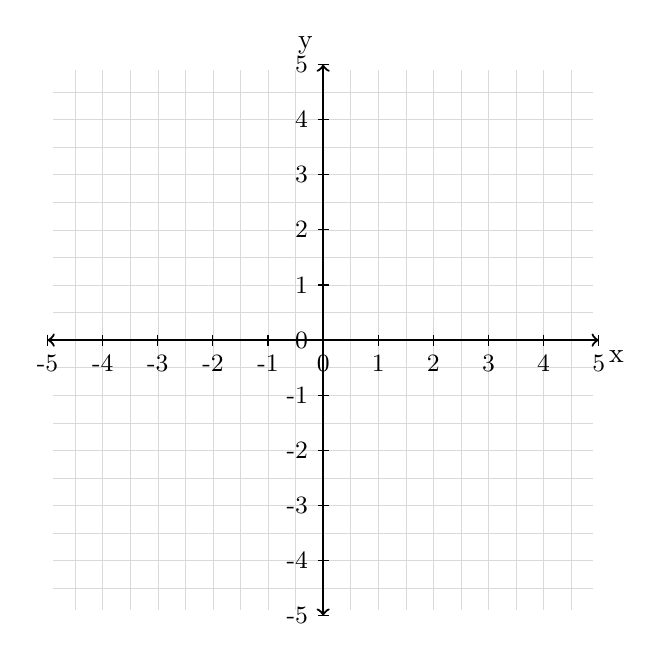
\begin{tikzpicture}[scale=0.7]
        \draw[gray!30, very thin, step=0.5] (-4.9,-4.9) grid (4.9,4.9);
        \draw[thick, <->] (-5,0) -- (5,0) node[below right] {x};
        \draw[thick, <->] (0,-5) -- (0,5) node[above left] {y};
        \foreach \x in {-5,-4,...,5} {
            \draw (\x,0.1) -- (\x,-0.1) node[below] {\small\x};
        }
        \foreach \y in {-5,-4,...,5} {
            \draw (0.1,\y) -- (-0.1,\y) node[left] {\small\y};
        }
    \end{tikzpicture}
    \end{center}
    
    Coordinates: \rule{3cm}{0.4pt}
    
    \item Start at (0, 0). Move right 3 units, then down 2.5 units. Plot your final position.
    
    \begin{center}
    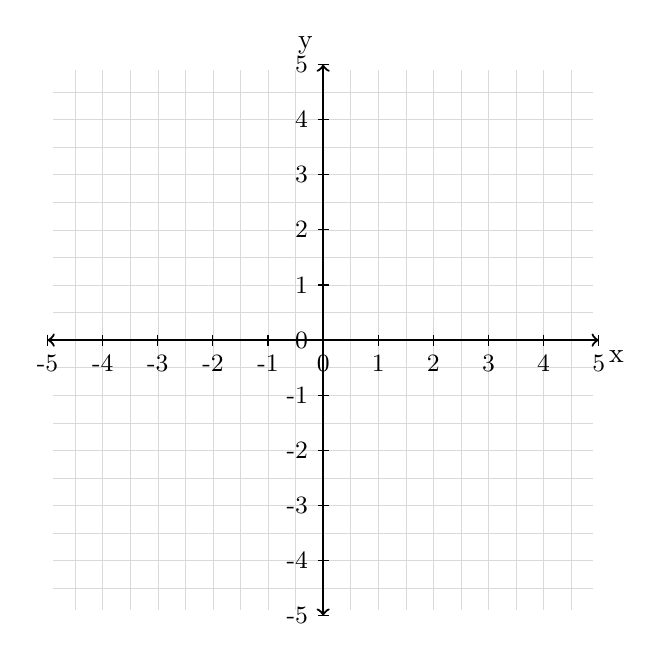
\begin{tikzpicture}[scale=0.7]
        \draw[gray!30, very thin, step=0.5] (-4.9,-4.9) grid (4.9,4.9);
        \draw[thick, <->] (-5,0) -- (5,0) node[below right] {x};
        \draw[thick, <->] (0,-5) -- (0,5) node[above left] {y};
        \foreach \x in {-5,-4,...,5} {
            \draw (\x,0.1) -- (\x,-0.1) node[below] {\small\x};
        }
        \foreach \y in {-5,-4,...,5} {
            \draw (0.1,\y) -- (-0.1,\y) node[left] {\small\y};
        }
    \end{tikzpicture}
    \end{center}
    
    Final coordinate: \rule{3cm}{0.4pt}
    
    \item Start at (-2, 1). Move left 1.5 units, then up 2 units. Plot your final position.
    
    \begin{center}
    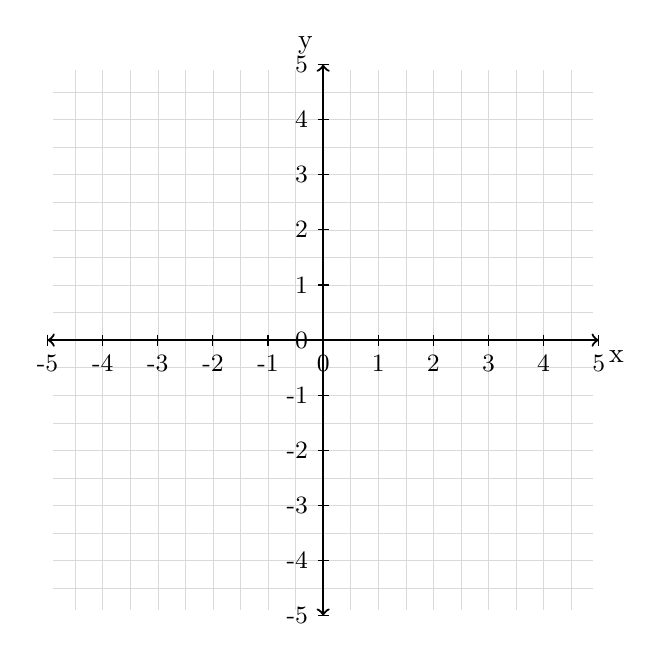
\begin{tikzpicture}[scale=0.7]
        \draw[gray!30, very thin, step=0.5] (-4.9,-4.9) grid (4.9,4.9);
        \draw[thick, <->] (-5,0) -- (5,0) node[below right] {x};
        \draw[thick, <->] (0,-5) -- (0,5) node[above left] {y};
        \foreach \x in {-5,-4,...,5} {
            \draw (\x,0.1) -- (\x,-0.1) node[below] {\small\x};
        }
        \foreach \y in {-5,-4,...,5} {
            \draw (0.1,\y) -- (-0.1,\y) node[left] {\small\y};
        }
    \end{tikzpicture}
    \end{center}
    
    Final coordinate: \rule{3cm}{0.4pt}
    
    \item A character starts at (0,0) facing 0° (to the right). They turn to face 90° (up) and move 2 units forward. Then they turn to face 180° (left) and move 1.5 units forward. Plot their initial and final position. Show the direction they move with an arrow.
    
    \begin{center}
    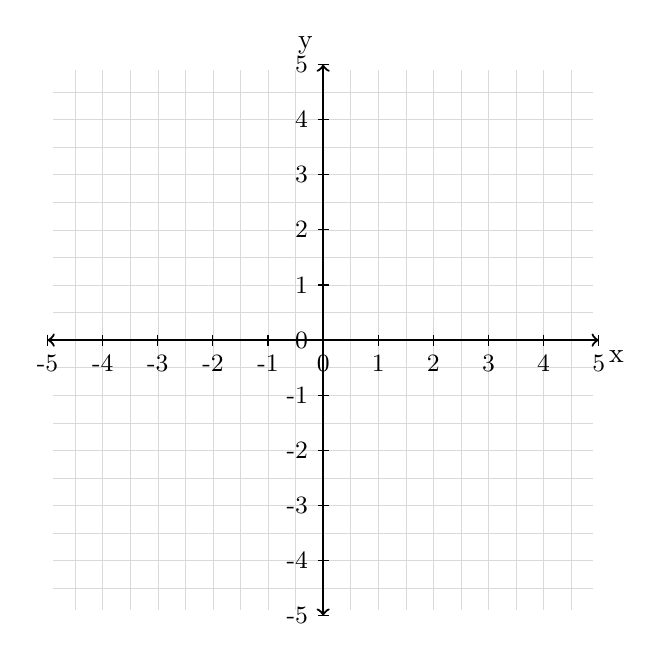
\begin{tikzpicture}[scale=0.7]
        \draw[gray!30, very thin, step=0.5] (-4.9,-4.9) grid (4.9,4.9);
        \draw[thick, <->] (-5,0) -- (5,0) node[below right] {x};
        \draw[thick, <->] (0,-5) -- (0,5) node[above left] {y};
        \foreach \x in {-5,-4,...,5} {
            \draw (\x,0.1) -- (\x,-0.1) node[below] {\small\x};
        }
        \foreach \y in {-5,-4,...,5} {
            \draw (0.1,\y) -- (-0.1,\y) node[left] {\small\y};
        }
    \end{tikzpicture}
    \end{center}
    
    Final coordinate: \rule{3cm}{0.4pt}
    
    \item A character starts at (1,1) facing -90° (down). They move down 2 units, then turn 90° counter-clockwise (now facing right) and move 3 units. Plot their initial and final position. Show the direction they move with an arrow.
    
    \begin{center}
    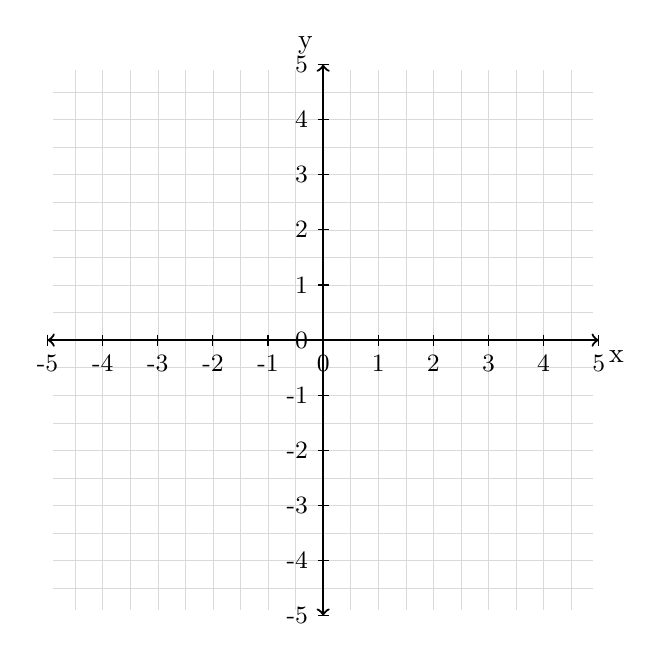
\begin{tikzpicture}[scale=0.7]
        \draw[gray!30, very thin, step=0.5] (-4.9,-4.9) grid (4.9,4.9);
        \draw[thick, <->] (-5,0) -- (5,0) node[below right] {x};
        \draw[thick, <->] (0,-5) -- (0,5) node[above left] {y};
        \foreach \x in {-5,-4,...,5} {
            \draw (\x,0.1) -- (\x,-0.1) node[below] {\small\x};
        }
        \foreach \y in {-5,-4,...,5} {
            \draw (0.1,\y) -- (-0.1,\y) node[left] {\small\y};
        }
    \end{tikzpicture}
    \end{center}
    
    Final coordinate: \rule{3cm}{0.4pt}
\end{enumerate}

\end{document}
